\chapter{Problem układania planu zajęć}
\section{Sformułowanie problemu}
Problem układania planu zajęć można sformułować następująco. Dana jest lista określonych wydarzeń, dostepnych okien czasowych i zasobów. Należy przyporządkować wydarzeniom okna czasowe oraz zasoby w taki sposób, by spełnić przyjęte założenia (rysunek 3.1). W formułowanym problemie:
\begin{itemize}
	\item wydarzeniami są poszczególne lekcje odbywające się w ciągu jednego tygodnia,
	\item dostępnymi oknami czasowymi są godziny w których mogą odbywać się zajęcia (np. od poniedziałku do piątku w godzinach między 8:00 a 18:00),
	\item zasoby to dostępne sale lekcyjne, nauczyciele prowadzący zajęcia, grupy uczniów itp.
\end{itemize}


\begin{figure}
	\centering
	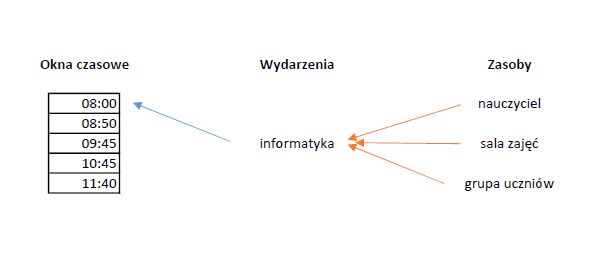
\includegraphics{podzialzasobow}
	\caption{Ilustracja problemu układania planu zajęć}
	\label{fig: podzialzasobow}
\end{figure}

Układanie planu zajęć wymaga spełnienia określonych ograniczeń. Mianowicie nie można wypełnić dostepnych okien czasowych według z góry przyjętej kolejności, ponieważ jest prawdopodobne, że pojawią się konflikty i plan zajęć nie będzie możliwy do zrealizowania. Aby tego uniknąć trzeba spełnić tzw. ograniczenia twarde, czyli takie, które zawsze muszą zostać spełnione, by plan mógł być możliwy do zrealizowania. Istnieją również ograniczenia miękkie, które określają jakość ułożonego planu. Ograniczenia te nie muszą zostać spełnione, ale algorytm układania planu zajęć powinien brać je pod uwagę.

\newpage
Przykłady ograniczeń:
\begin{itemize}
	\item twarde:
	\begin{itemize}
		\item zasób nie może być wykorzystany w dwóch miejscach w tym samym czasie (np. dany nauczyciel nie może prowadzić jednocześnie zajęć w dwóch różnych salach),
		\item nie występują zajęcia, które nie zostały przypisane do okien czasowych w ułożonym planie.
	\end{itemize}
	\item miękkie:
	\begin{itemize}
		\item brak dłuższych przerw między zajęciami dla uczniów,
		\item odpowiednie przerwy między zajęciami (np. 15 - lub 20 - minutowe),
		\item liczba dni roboczych, w których nauczyciele prowadzą zajęcia, powinna być minimalizowana,
		\item brak bloków zajęć danego typu (np. dana grupa uczniów nie powinna mieć kolejno czterech lekcji matematyki).
	\end{itemize}
\end{itemize}

%Niepodzielność zasobów oznacza, że jeden nauczyciel nie może być w dwóch miejscach jednocześnie, więc może prowadzić tylko jedne zajęcia w danym oknie czasowym, w jednej sali nie mogą się odbywać w tym samym czasie różne zajęcia, a dla danej grupy lekcje nie mają prawa się nakładać. Naruszenie tego ograniczenia było by fizycznie nie możliwe. 
%Obowiązek przypisania zajęć do jakichś okien czasowych oznacza, że na planie końcowym muszą się znaleźć wszystkie lekcje przewidziane w siatce zajęć dla danej grupy. Jest to podstawowe założenie bez którego układanie planu traci swój sens.
Często jednak dla wyjściowej siatki zajęć spełnienie wymagań twardych jest niemożliwe. Wynika to najczęściej z za małej liczby zasobów (za mało nauczycieli mogących prowadzić jeden przedmiot lub za mało sal). W algorytmach szuka się wtedy planu z najmniejszą liczbą niespełnionych wymagań, które są usuwane ręcznie przez szukanie określonych kompromisów (np. dołożenie okna czasowego, zatrudnienie dodatkowego nauczyciela, zaplanowanie zajęć tego samego typu dla dwóch mniejszych grup w jednej sali).

Ograniczenia miękkie to w istocie życzenia nauczycieli i uczniów co do tego jak  plan powinien wyglądać. Niespełnienie tych ograniczeń wpływa na końcową ocenę planu zajęć, niespelnione ograniczenia mogą mieć określone wagi w zależności od ich istotności. Niektóre plany zajęć układane są ze szczególnym uwzględnieniem uczniów (mała liczba okienek, równomierne rozłożenie zajęć, brak bloków zajęć tego samego typu, odpowiednia przerwa między zajęciami), a niektóre z uwzględnieniem potrzeb prowadzących (zajęcia skumulowane w ciągu dwóch dni tygodnia by umożliwić prace w innej szkole). Założenia te z reguły precyjzuje osoba uruchomiająca wykonanie planu przez odpowiednie skonfigurowanie parametrów algorytmu i zdefiniowanie funkcji oceny wygenerowanego planu.

Funkcja oceny planu zajęć z reguły przewiduje nakładanie punktów karnych za niespełnienie określonych ograniczeń. Każde ograniczenie ma ustaloną liczbę punktów karnych, przy czym ograniczenia twarde powinny mieć dużo większą wagę od ograniczeń miękkich. Im więcej punktów karnych ma plan tym jest gorszy. To właśnie na podstawie funkcji oceny planu większość algorytmów starta się ułożyć jak najlepszy plan zajęć.

\section {Rozmiar problemu}

By dobrze zrozumieć potrzebę używania algorytmów heurystycznych przy wyszukiwaniu najlepszego planu zajęć warto przybliżyć pojęcie skali problemu. W tym celu przedstawimy przykład planu zajęć dla amerykańskiej szkoły średniego rozmiaru. W przykładzie tym, każde ze zdarzeń ma przyporządkowane wcześniej zasoby. Przykład ten zawiera:

\begin{itemize}
	\item okna czasowe - 40,
	\item nauczyciele - 27,
	\item sale - 30,
	\item grupy uczniów - 24,
	\item zdarzenia - 832,
	\item ograniczenia - 4.
\end{itemize}

Dostępnych jest 40 okien czasowych, które rozłożone na pięć dni zajęć w tygodniu dają osiem godzin zajęć dziennie. Jednocześnie odbywać się mogą 24 zajęcia. Liczba ta wynika z niepodzielności zasobów i jest minimalną liczbą spośród liczby nauczycieli, sal i grup uczniów. Maksymalna liczba zdarzeń, które mogą się odbywać w danym tygodniu wynosi więc:
\[ 40 \cdot 24 = 960, \]
\[ 960 > 832. \]
Maksymalna liczba zdarzeń jest większa od liczby zdarzeń zawartych w siatce zajęć podanego przykładu, więc realizacja  planu zajęć zgodnego z powyższą specyfikacją zasobów jest możliwa.

Na jedną grupę uczniów przypada około 35 zdarzeń (832/24), które powinny być rozłożone na 40 okien czasowych. Uwzględniając możliwość wystąpienia okienek w trakcie zajęć, mamy więc 40-wyrazowy ciąg zdarzeń. Liczba możliwości, w które można te zajęcia rozłożyć, określa liczba permutacji 40!, która wynosi:
\[40! = 815915283247897734345611269596115894272000000000\]
Jest to 48 cyfrowa liczba możliwości rozłożenia zajęć w oknach czasowych dla jednej grupy. Liczbę tę trzeba pomnożyć przez liczbę grup.

Liczba możliwości może być jeszcze większa, jeżeli uwzględnimy to, że każde zajęcia mogą mieć przypisanego dowolnego nauczyciela z grupy osób uprawnionych do prowadzenia przedmiotu. Również sale zajęć mogą być różne dla danego wydarzenia. By zmniejszyć tę liczbę możliwości, odpowiednio modyfikuje się dane wejściowe. Każde zajęcia (zdarzenia) w danych wejściowych, mogą mieć przypisane na stałe zasoby takie jak sala, grupa i nauczyciel. Szukaną niewiadomą jest wtedy tylko termin odbywania się zajęć. Dzięki temu przestrzeń możliwych rozwiązań dla algorytmu układania planu zajęć zmniejsza się. Dodatkowo przypadek, w którym każde zajęcia mają wcześniej przypisanego prowadzącego, ma odzwierciedlenie w potrzebach współczesnych szkół, gdzie wyspecjalizowana kadra zatrudniana jest często w niepełnym wymiarze godzin, przez to może być przydzielona tylko do wybranej ilości zajęć.

Podejście, w którym zasoby, takie jak sala i nauczyciel, są przypisane z góry do zdarzeń, umożliwia szybsze działanie algorytmu. Jednak trzeba pamiętać, że ma to również wpływ na wynik końcowy. Może się zdarzyć przypadek, w który nie istnieje możliwość ułożenia optymalnego planu dla danych wejściowych, a wystarczyło by zamienić nauczyciela przypisanego do jednych zajęć, z innym nauczycielem tego samego przedmiotu, by odblokować nowe możliwości. Jednak z uwagi na czas działania algorytmu, jak i na dostępne dane testowe, zdecydowano się wybrać wariant, w którym do algorytmu przekazywane są zdarzenia z przypisanymi nauczycielami, salami oraz grupami, a algorytm wyszukuje tylko odpowiednie okna czasowe dla podanych zdarzeń.